\section{Optimisation discrète}

\begin{enumerate}

  \item Considérez le problème d'optimisation en nombres entiers

    $
    \begin{array}{lrcrcl}
      \maxi & 5x_1 & +&  x_2\\
      & -x_1 &+& 2 x_2  & \leq & 4 \\
      & x_1    & - &    x_2   &  \leq & 1\\
      &   4x_1& +&  x_2  & \leq & 12 \\
      &   \multicolumn{3}{r}{x_1, x_2}  & \geq & 0\\
      &   \multicolumn{3}{r}{x_1, x_2}  & \multicolumn{2}{l}{\mbox{ entiers}}
    \end{array}
    $

    Trouvez graphiquement une solution de ce problème. Trouvez graphiquement une solution optimale du problème relaxé. Trouvez la
    solution entière la plus proche de la solution optimale du problème relaxé. Enumérez toutes le solutions entières obtenues en
    arrondissant la solution optimale du problème relaxé. Une de ces solutions est-elle optimale?


    \begin{solution}
      En analysant le graphique, la solution $x = (2,3)$ est optimale parmi les solutions admissibles entières.
    \end{solution}

  \item Yves et Muriel désirent partager les principales tâches ménagères  (courses, cuisine, vaisselle et nettoyage)
    entre eux. Leurs efficacités à la réalisation de ces tâches
    diffèrent. Yves est rapide pour faire les courses et la vaisselle mais il se fait distancer par Murielle pour la cuisine et le
    nettoyage.

    $
    \begin{array}{l|llll}
      & courses & cuisine & vaisselle & nettoyage\\
      \hline
      Yves & 4.5 & 7.8 & 3.6 & 3.1\\
      Muriel & 4.9 & 7.2 & 4.3 & 2.9
    \end{array}
    $

    Le jeune couple  désire partager les tâches de manière équitable (deux tâches par personne) et optimale (temps total minimum). Formulez
    ce problème comme un problème d'optimisation en nombres entiers. Donnez une relaxation de ce problème. La solution du problème
    relaxé est-elle entière? Que pouvez-vous en déduire?


    \begin{solution}
      Le problème devient : \\
      $$ \min \sum_{ij}c_{ij}x_{ij}$$
      sous les contraintes \\
      $$ \sum_{j} x_{ij} = 2 \qquad i = 1,2$$
       $$ \sum_{i} x_{ij} = 1\qquad j = 1, \dots,4$$
       $$x_{ij} \in \lbrace 0,1\rbrace$$
    \end{solution}

  \item Vouz désirez choisir un ensemble de cours parmi huit cours $\{1, \ldots,
    8 \}$ pour vous constituer un programme. Modélisez les contraintes
    suivantes:

    \begin{enumerate}
      \item Vous ne pouvez pas choisir plus de 5 cours mais devez en choisir au
        moins 3.
      \item Le cours 3 est un prérequis du cours 6 et le cours 2 un prérequis
        du cours 7.
      \item Les cours 8 et 6 forment une paire. Vous devez les prendre tous les
        deux, ou aucun des deux.
      \item Pour des questions de conflit horaire, vous ne pouvez pas choisir
        les cours 5 et 2, ni les cours 3 et 6.
      \item Pour vous conformer aux contraintes de votre programme d'étude vous devez choisir au moins un des cours
        1, 2, 3 ou au moins deux cours parmi les cours 5, 6, 7, 8.
    \end{enumerate}


    \begin{solution}
       (a) $3 \le \sum_{i} x_{i} \le 5$ \\
       \newline
       (b) $x_{6} \le x_{3}$ et $x_{7} \le x_{2}$ \\
        \newline
       (c) $x_{6} = x_{8}$ \\
        \newline
       (d) $x_{2} + x_{5} \le 1$ et $x_{3} + x_{6} \le 1$\\
        \newline
      (e) $ 1-y \le x_{1} + x_{2} + x_{3} \le 3(1-y)$ et $ 2y \le x_{5} + x_{6} + x_{7} + x_{8} \le 4y$ où $y \in \lbrace 0,1\rbrace$.
    \end{solution}

  \item Vous désirez trouver les variables $0 \leq x_1, x_2 \leq 1$ qui maximisent la fonction $c^T x$ tout en satisfaisant au
    moins une  des deux contraintes $x_1 + 2 x_2 \leq 1$  et  $3 x_1 +  x_2 \leq 1$. Formulez ce problème comme un
    problème d'optimisation mixte.



    \begin{solution}
      Néant
    \end{solution}

  \item Une société a développé deux nouveaux jouets pour la Noël. La production du jouet 1 nécessite des investissements initiaux de
    50000 EUR et celle du jouet 2 des investissements initiaux de 80000 EUR. Les jouets
    génèrent un profit de 10 EUR pour le jouet 1 et de 15 EUR pour le jouet 2.  Le jouet 1 est
    produit à un taux de 50 l'heure et le jouet 2 à un taux de 25 l'heure. On dispose  de 500 heures
    d'ici Noël. Déterminez le nombre de jouets à produire de manière à maximiser le profit.


    Supposons maintenant que la société possède deux usines. Une seule usine sera choisie pour la production. Le
    jouet 1 est produit à un taux de 50 l'heure dans l'usine 1 et de 40 l'heure dans l'usine 2. Le jouet 2 est produit à un taux de
    25 l'heure dans les deux usines. Les usines disposent de 500 et 700 heures d'ici Noël.  Le problème consiste à déterminer le
    nombre de jouets à produire de manière à maximiser le profit.












    \begin{solution}
    \end{solution}

  \item Vous disposez de 4 objets de poids respectifs 5, 3, 8 et 7. Les utilités des
    objets sont de 17, 10, 25 et 7. Vous désirez sélectionner un ensemble d'objets de poids total inférieur  à 12 et dont la somme
    des utilités est maximale.  Formulez le problème comme un problème d'optimisation en nombres entiers. Trouvez la solution.


    \begin{solution}
      Comme il s'agit de variables binaires, il y a au plus $2^{4}$ possibilités avant de trouver la solution optimale. La \textit{stratégie} efficace consiste à annuler les variables dont le rapport entre utilité/poids est le plus faible. On obtiendra une valeur qui s'approche de la fonction coût du problème relaxé. En testant les autres branches dont les coûts sont supérieurs, on trouve finalement $x = (0,1,1,0)$.
    \end{solution}

  \item Vous disposez de 5 objets de poids respectifs 2, 4, 3, 3 et 2. Les
    utilités des objets sont respectivement de 9, 20, 14, 10 et 6. Vous désirez
    sélectionner un ensemble d'objets de poids total inférieur  à 10
    et dont la somme des utilités est maximale.  Formulez le problème
    comme un problème d'optimisation en nombres entiers. Appliquez l'algorithme ``branch and bound" pour trouver la
    solution. Justifiez les étapes de l'algorithme.


    \begin{solution}
    \end{solution}

  \item  Considérez l'arbre d'énumération suivant pour un problème d'optimisation en nombres entiers. L'arbre
    résulte-t-il d'un problème de maximisation ou de minimisation?  Quels sont les noeuds qui doivent encore être analysés? Donnez
    un intervalle dans lequel se trouve l'optimum. Que pouvez vous dire de la solution optimale?








    \begin{solution}
    \end{solution}

  \item Considérez le problème d'optimisation en nombres entiers

    $
    \begin{array}{lrcrcl}
      \maxi & 9x_1 & +&  5 x_2\\
      & 4 x_1 &+& 9 x_2  & \leq & 35 \\
      & x_1    &  &       &  \leq & 6\\
      &   x_1& -&  3x_2  & \geq & 1 \\
      & 3 x_1    & + & 2x_2   &  \leq & 19\\
      &   \multicolumn{3}{r}{x_1, x_2}  & \multicolumn{2}{l}{\mbox{ entiers}}
    \end{array}
    $


    Résolvez le problème graphiquement et algébriquement en utilisant la méthode ``branch and bound".



    \begin{solution}
      En observant la fonction coût, on constate qu'il est plus avantageux de donner la plus grande valeur entière possible à $x_{1}$ car le coefficient est supérieur à celui de $x_{2}$. On obtient $x = (6,0)$. On peut régresser pour $x_{1} = 5$, mais on s'aperçoit que la fonction coût décroît.
    \end{solution}

  \item Considérez l'arbre d'énumération suivant pour un problème d'optimisation de deux variables entières.

    \begin{enumerate}
      \item L'arbre résulte-t-il d'un problème de maximisation ou de minimisation?
      \item \label{r1} Quels sont les
        noeuds qui doivent encore être analysés?
      \item \label{r2} Donnez un intervalle dans lequel se trouve
        l'optimum.
      \item La fonction objectif est donnée
        par $3x_1+6x_2$. Cette information vous permet-elle de préciser vos réponses aux sous-questions \ref{r1} et
        \ref{r2}?
    \end{enumerate}


    \begin{solution}
    \end{solution}

  \item  Il y a 50 groupes d'étudiants en première candidature FSA. On souhaite affecter un projet par groupe. Il y a 10
    projets disponibles et chaque projet peut être affecté à au plus 10 groupes. On a demandé à chaque groupe de classer les trois projets qui ont leur
    préférence. On souhaite affecter à chaque groupe un des projets qu'il a classés et maximiser le nombre de groupes qui recoivent leur premier choix.
    S'il y a plusieurs affectations qui satisfont cette contrainte, on souhaite, parmi l'ensemble de ces affectations, choisir celle qui maximise le nombre de groupes
    qui recoivent leur deuxième choix. Vous êtes coordinateur d'année en FSA; proposez une manière de résoudre ce problème.


    \begin{solution}
    \end{solution}

  \item Le Sudoku est un jeu logique présenté sous forme de grille. D'abord publié en 1979, le Sudoku s'est développé au Japon en 1986 avant d'atteindre la popularité internationale en 2005, et ce jusqu'aux colonnes de l'hebdomadaire ``la Salopette" édité par le CI. La grille de jeu est un carré de neuf cases de côté, subdivisé en neuf carrés, appelés régions (voir figure). Quelques chiffres sont disposés dans la grille et le but du jeu est de compléter la grille avec des chiffres  de un à neuf en respectant la règle suivante: chaque ligne, colonne et région ne doit contenir qu'une et une seule fois  les chiffres de un à neuf.

    \begin{enumerate}

      \item Formulez le problème du Sudoku pour une grille quelconque comme un problème  d'optimisation linéaire en nombres entiers.

      \item Une grille de Sudoku peut ne pas avoir de solution. Si une grille ne possède pas de solution, un objectif naturel consiste à compléter  toutes les cases de manière à ce que le nombre total de lignes, colonnes et régions complètes soit aussi élevé que possible (une ligne, colonne ou région est complète si tous les nombres de un à neuf y apparaissent exactement une fois). Formulez ce problème comme un problème d'optimisation linéaire en nombres entiers.

        \begin{center}
          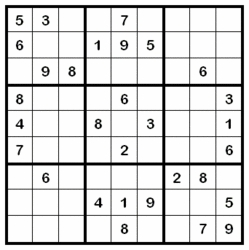
\includegraphics[scale=0.7]{sudo.jpg}
        \end{center}

    \end{enumerate}

    \begin{solution}
      Néant
    \end{solution}

  \item \textsc{OptiTv} lance un nouveau jeu sur nos écrans.  La
    dernière épreuve du jeu permet au gagnant de
    multiplier ses gains.

    Deux rails $A$ et $B$ traversent un plateau de jeu jonché
    d'obstacles.  Le but du joueur est de maximiser la masse
    totale
    de deux billes posées sur les rails qui pourront traverser le plateau.
    Pour ce faire, il peut décider de retirer
    certains obstacles du parcours, mais pour chaque obstacle
    enlevé, une pénalisation de $20$ grammes lui sera retranchée du résultat.
    Les règles du jeu sont les suivantes:
    \begin{enumerate}
      \item Le joueur a à sa disposition des billes de $10$,
        $20$, $30$, ..., $100$ grammes en quantité suffisante.  Il
        peut déposer $0$, $1$ ou $2$ billes sur le plateau
        (maximum une bille par rail), et chaque bille déposée doit
        traverser de part en part le plateau sous peine de
        disqualification.
      \item Pour assurer l'équilibre du plateau, la différence
        de masse entre les deux billes choisies ne peut pas excéder
        $20$ grammes. En particulier, si une seule bille traverse le
        plateau, sa masse ne peut pas être supérieure à $20$
        grammes.
      \item Si l'obstacle $1$ n'est pas ôté, une bille posée sur le rail $A$ ne
        peut pas traverser le plateau de jeu.
      \item Les obstacles $2$ et $3$ ne peuvent pas être retirés
        tous les deux ensemble.
      \item S'il souhaite retirer l'obstacle $2$ ou l'obstacle
        $4$, le joueur est obligé d'enlever d'abord les obstacles
        $1$ et $3$.
%        {\it \item Le joueur est obligé d'enlever au moins un des
%        obstacles parmi $2$ et $4$ ou d'enlever les deux obstacles
%        $1$ et $3$.}
      \item Les obstacles $3$ et $4$ déterminent conjointement
        la masse maximale de la bille qui pourra passer sur le rail $B$: le
        retrait de l'obstacle $3$ permet de faire passer $80$
        grammes et le retrait de l'obstacle $4$ autorise quant à lui $20$
        grammes.  En particulier, si ces deux obstacles sont
        retirés, une bille de $100$ grammes peut passer sur ce
        rail.
        %Quatre obstacles peuvent gêner la progression des billes.
    \end{enumerate}

    Formulez ce problème comme un problème d'optimisation linéaire
    en nombres entiers.  Vous ne devez pas résoudre ce
    problème.




    \begin{solution}
    \end{solution}

  \item Vous disposez d'une somme de 96 Euros. Vous désirez acheter
    des boissons, disponibles en divers conditionnements.
    \begin{center}
      \begin{tabular}{|c|c|c|c|c|c|}
        \hline %\vspace{2pt}
        Boisson & A & B & C & D & E\\
        \hline
        Volume unitaire (litres) & 15 & 16 & 17 & 18 & 20\\
        \hline
        Prix unitaire (Euros) & 16 & 17 & 18 & 19 & 20\\
%\hline Nombre disponible & $\infty$ & $\infty$ & 6  & 4\\
        \hline
      \end{tabular}
    \end{center}
    Vous désirez acheter un volume le plus grand possible, sans
    dépasser votre budget.
    \begin{enumerate}
      \item Formulez ce problème comme un problème d'optimisation
        linéaire en nombres entiers.
      \item Combien de conditionnements de chaque type allez-vous acheter
        ? Détaillez votre raisonnement.
    \end{enumerate}

    \begin{solution}
    \end{solution}

  \item Un transporteur est confronté au problème suivant : il ne
    peut transporter qu'une tonne de marchandises dans son véhicule,
    alors qu'une quantité supérieure à une tonne est disponible. Il
    reçoit les données suivantes de la part du comptable de
    l'entreprise, regroupant les quantités disponibles de chaque
    marchandise, ainsi que le bénéfice retiré par leurs ventes
    respectives.

    \begin{center}
      \begin{tabular}{|c|c|c|c|}
        \hline %\vspace{2pt}
        Marchandise & A & B & C\\
        \hline
        Quantité disponible (kg) & 900 & 240 & 560 \\
        \hline
        Bénéfice (euros/kg) & 15 & 17,5 & 14 \\
        \hline
      \end{tabular}
    \end{center}

    \begin{enumerate}
      \item D'après ces informations, formulez le problème d'optimisation
        linéaire correspondant et déterminez les quantités de A,B et C qui
        optimiseront le bénéfice réalisé par la vente du chargement et
        donnez la valeur de ce bénéfice.

        \vspace{6pt} Arrivé dans le hangar pour charger, le chauffeur
        réalise que les marchandises sont conditionnées en sacs, et qu'il
        est impensable de charger autres choses que des sacs complets.
        Voici les poids des sacs qui constituent le stock :
        \begin{center}
          \begin{tabular}{|c|c|c|c|}
            \hline %\vspace{2pt}
            Marchandise & A & B & C\\
            \hline
            Poids d'un sac (kg) & 60 & 80 & 20 \\
            \hline
          \end{tabular}
        \end{center}

      \item Reformulez le problème d'optimisation en tenant compte de ces
        dernières informations. Résolvez ce nouveau problème et comparez
        votre solution à la solution du cas~(a). Justifiez votre
        raisonnement.

      \item Le chauffeur (décidément malchanceux) se rend compte que le
        comptable a oublié de mentionner la marchandise D dont il reste
        trois sacs de 50 kg pouvant rapporter chacun 1000 Euros. A ce
        moment, il a déjà chargé neuf sacs de A et deux sacs de B, et ne
        compte pas les enlever de sa camionnette. Formulez le nouveau
        problème d'optimisation et expliquez une méthode de résolution
        "systématique" (par opposition à intuitive) de ce problème, sans la
        mener à terme.
    \end{enumerate}



\end{enumerate}




\end{document}




\newpage





%******************************************************************************



\section{Optimisation non-linéaire: Gradient et gradients conjugués}



\begin{enumerate}

    \begin{solution}
    \end{solution}

  \item Soit la fonction $f(x_1, x_2)= 2 x_1^3+3 x_1^2+12x_1 x_2 + 3 x_2^2
    -6 x_2 + 54$. Trouvez les points stationnaires de cette fonction et déterminez leur nature.
    La fonction possède-t-elle un minimum global? un maximum global?

    \begin{solution}
    \end{solution}

  \item Trouvez les points maximants et les points minimants de la fonction $f(x_1, x_2)=2x_1^2+x_2^2-2x_1x_2+2x_1^3+x_1^4$.

    \begin{solution}
    \end{solution}

  \item Trouvez si possible une fonction $f$ de deux variables et un point stationnaire $x_*$ de $f$ qui maximise $f$ et pour lequel
    $\nabla^2 f(x_*)
    \geq 0$. Même question pour  $\nabla^2 f(x_*)> 0$

    \begin{solution}
    \end{solution}

  \item Considérez la fonction quadratique $f(x)=(1/2) x^T Q x-c^T x$ avec $Q$ symétrique. Sous quelle condition cette fonction possède-t-elle un
    point stationnaire? un minimum local? un point stationnaire mais pas de minimum ni de maximum local?

    \begin{solution}
    \end{solution}

  \item Soit $f(x_1, x_2)=2x_1^2+x_1 \sin x_2$ la direction $(-2, 3)$ est-elle une direction de descente pour $f$ en $(2, -1)$? Si oui, donnez
    une expression pour le point résultant de la minimisation de la fonction dans cette direction.


    \begin{solution}
    \end{solution}

  \item On d\'esire minimiser la fonction:

    $$
    f(x_1, x_2)=2x_1^2 + x_2^2 - 2xy + 2x_1^3 + x_1^4
    $$

    par une methode it\'erative. Celle-ci nous am\`ene \`a minimiser
    la fonction objectif le long de la direction $d = (-1, 4)^T$ au
    d\'epart du point $x=(2,-1)^T$. La direction $d$ est-elle une
    direction de descente? Utilisez la condition d'Armijo pour trouver
    un nouveau point de d\'epart.


%SOLUTION:
%
%gradient = $(66, -6)$ donc descente. Il faut minimiser
%$f(2-\alpha, -1+ 4* \alpha)$. Avec $\epsilon=0.1$ (donc Armijo est
%$f(x+ \alpha*d) \leq 45 - 9*\alpha$) et $\eta=2$, $\alpha=1$
%convient.


    \begin{solution}
    \end{solution}

  \item Soit la fonction $f(x,y)=x^2+y^2(x^4-5x^2+7)$. Lors d'une
    tentative de minimisation de cette fonction, on utilise un
    algorithme qui essaie successivement comme directions de descente
    les axes $x$ et $y$.
    \begin{enumerate}
      \item Considérant une descente suivant l'axe $x$ à partir du point
        $(2,2)$, déterminez le sens de descente (augmentation ou
        diminution de $x$). Justifiez.
      \item Ayant obtenu la direction de
        descente $d_k$ au point précédent, on définit la fonction
        $F(\alpha)=f(x_k-\alpha d_k)$. Utilisez le critère d'Armijo pour
        effectuer une minimisation approximative de la fonction
        $F(\alpha)$. Donnez le $\alpha$ obtenu, ainsi que les coordonnées
        du point atteint.
      \item Appliquez maintenant la méthode en utilisant
        la direction $y$ à partir du nouveau point obtenu.
    \end{enumerate}

%%Réponse:
%%\begin{enumerate}
%%\item Direction : $(-1,0)$, car $\nabla f (2,2) = (52,12)$.
%%\item $F(\alpha)=f(2-\alpha,2)=4(2-\alpha)^4-19(2-\alpha)^2+28$.
%%\newline $F(0)=16$, $F'(0)=-52$
%%\newline Critère d'Armijo, avec $\varepsilon=1$ : $F(\alpha)\leq 16-5.2 \alpha$
%%\newline Essai avec $\alpha=1$ ok, $\alpha=2$ non. Donc
%%$\alpha=1$.
%%\newline Point atteint : (1,2)
%%\item $F(\alpha)\leq 13-1.2 \alpha$, $\alpha=2$, (1,0)
%%\newline puis en $x$, $F(\alpha)\leq 1-0.2 \alpha$, $\alpha=1$, (0,0).





    \begin{solution}
    \end{solution}

  \item Soit $f(x_1, x_2)=2x_1^2 + x_2^2 -2 x_1 x_2 + 2 x_1^3 + x_1^4$. La direction $(0, 1)$ est-elle une direction de descente pour $f$ en
    $(0, -2)$? Trouvez l'ensemble des directions de descente en ce point. Quelle est la direction de plus grande pente?

    \begin{solution}
    \end{solution}

  \item Soit $f$ une fonction dont on cherche un minimum au moyen d'un algorithme qui effectue des minimisations unidimensionnelles exactes.
    Démontrez qu'une direction de recherche $d_k$ est toujours orthogonale au gradient de la fonction au nouveau point $x_{k+1}$.

    \begin{solution}
    \end{solution}

  \item Soit la fonction quadratique $f(x)=(1/2) x^T Q x-c^T x$ avec $Q=diag(1, \gamma, \gamma^2)$ et $c=(1, 1, 1)^T$. On cherche un minimum
    de $f$ au moyen de la méthode de la plus grande pente au départ de l'origine. Pouvez-vous borner le nombre d'itérations en fonction de la
    précision souhaitée?

    \begin{solution}
    \end{solution}

  \item La méthode de la plus grande pente est appliquée au problème de la minimisation de $f(x_1, x_2)=x_1^2 + 2 x_2^2$ au départ de $(2, 1)$.
    Montrez que les approximations successives sont données par $x_k =  (2, (-1)^k)/3^k$. Montrez que $f(x_{k+1})=f(x_k)/9$.


    \begin{solution}
    \end{solution}

  \item  La fonction de Rosenbrock est la fonction

    $$f(x_1,x_2) = (x_1-1)^2 + \lambda({x_1}^2-x_2)^2$$

    pour $\lambda \in \R$.\\



    a) Trouvez les points stationnaires de $f$ et discutez leur nature en fonction de $\lambda$.\\

    b) La méthode de la plus grande pente est utilisée pour trouver un point minimant de $f$ au départ de $(0, 0)$.
    Combien d'itérations faut-il dans le cas $\lambda = 0$? Caractérisez la vitesse de convergence de la
    méthode dans le cas $\lambda >0$. Si possible, quantifiez votre réponse pour le cas  $\lambda =10$.

    \begin{solution}
    \end{solution}

  \item  Consid\'erons la fonction

    $$f(x_1,x_2) = 5 x_1^2 + 3 x_1 x_2 + 5 x_2^2 - 6 x_1 -8 x_2$$




    a) Trouvez les points stationnaires de $f$ et discutez leur nature.

    b) La m\'ethode de la plus grande pente est utilis\'ee pour trouver un point
    minimant de $f$ au d\'epart de $(0, 0)$.
    Caract\'erisez la vitesse de convergence de la
    m\'ethode. Si possible, quantifiez votre r\'eponse.



\end{enumerate}

%******************************************************************************




\newpage


\section{Optimisation non-linéaire: Newton et quasi-Newton}

\begin{enumerate}



    \begin{solution}
    \end{solution}

  \item Utilisez la méthode de Newton pour trouver un point minimant de $f(x_1, x_2)=5x_1^4+6x_2^4-6x_1^2+2 x_1 x_2 +5x_2^2+15x_1-7x_2+13$.
    Partez de $x_0=(1, 1)$.

    \begin{solution}
    \end{solution}

  \item Utilisez la méthode de Newton modifiée (avec une recherche unidimensionnelle) pour la résolution de
    $$\min 2x_1^2 + x_2^2-2x_1 x_2 + 2 x_1^3 + x_1^4$$
    Effectuez seulement les deux premières
    itérations et partez de $x_0=(2, -1)$.



    \begin{solution}
    \end{solution}

  \item Appliquez la méthode de quasi-Newton de rang un à la résolution de

    $$\min \frac{1}{2} x^TAx-b^Tx$$ pour

  $$A=\left( \begin{array}{rrr} 5 & 2& 1 \\ 2 & 7 & 3 \\ 1 & 3 & 9 \end{array} \right) \quad  b= \left( \begin{array}{c} -9 \\ 0 \\8
    \end{array} \right).$$

    Initialisez la méthode avec $x_0= (0, 0, 0)$ et $H_0 = I$.



    \begin{solution}
    \end{solution}

  \item  Démontrez qu'avec la méthode Davidon-Fletcher-Powell tout  choix
    de $\alpha_k>0$ pour lequel $p_k^T q_k >0$ est tel que $H_{k+1}$ est définie positive lorsque $H_k$ l'est. Montrez que cette propriété est bien
    satisfaite lorsque $\alpha_k$ est le point minimant de $F(\alpha)=f(x_k+ \alpha d_k)$. Vous pouvez utiliser le fait que toute matrice
    symétrique et définie positive $A$ possède une racine carrée $B$ symétrique et définie positive, $A= B B$ avec $B$ symétrique et
    définie positive.

    \begin{solution}
    \end{solution}

  \item Nous considérons la méthode DFP. Supposons que la fonction $F(\alpha)= f(x_k+ \alpha d_k)$  possède unique minimum $\alpha'$ et est
    dérivable pour
    $\alpha >0$. Démontrez que tout choix de $\alpha_k > \alpha'$ pour $x_{k+1}=x_k + \alpha_k d_k$ est tel que
    $p_k^T q_k >0$.

    \begin{solution}
    \end{solution}

\end{enumerate}
